%!TEX TS-program = xelatex
%!TEX encoding = UTF-8 Unicode

% Copyright (C) 2014 Chen-Pang He <jdh8@ms63.hinet.net>
%
% This file is free software: you can redistribute it and/or modify
% it under the terms of the GNU General Public License as published by
% the Free Software Foundation, either version 3 of the License, or
% (at your option) any later version.
%
% This file is distributed in the hope that it will be useful,
% but WITHOUT ANY WARRANTY; without even the implied warranty of
% MERCHANTABILITY or FITNESS FOR A PARTICULAR PURPOSE.  See the
% GNU General Public License for more details.
%
% You should have received a copy of the GNU General Public License
% along with this program.  If not, see <http://www.gnu.org/licenses/>.

\documentclass{beamer}
\usepackage{metalogo}
\usepackage{xeCJK}

\hypersetup{colorlinks,linkcolor=,unicode}
\useoutertheme{sidebar}
\usecolortheme{rose}
\usecolortheme{seahorse}

\setCJKmainfont{WenQuanYi Micro Hei}

\title{Google 日曆}
\subtitle{物盡其用篇}
\author[何震邦]{何震邦 \textless jdh8@ms63.hinet.net\textgreater\\[1em]
    \href{https://creativecommons.org/licenses/by-sa/3.0/tw/deed}{\includegraphics{by-sa.eps}}}
\date{2013 年 9 月 12 日}

\begin{document}
\maketitle

\section{序}
\subsection{版權宣告}
\begin{frame}{版權宣告}
  \begin{itemize}
    \item 文字部份以 \href{https://creativecommons.org/licenses/by-sa/3.0/tw/deed}{CC-BY-SA 3.0} 方式釋出
    \item 來自 Google 日曆的圖像作示範用途,為合理使用
    \item 本簡報完全以自由軟體製作
    \begin{description}
      \item[字型] \href{https://zh.wikipedia.org/wiki/Computer\textunderscore Modern}{Computer Modern} +
        \href{http://wenq.org/wqy2/index.cgi?MicroHei}{文泉驛微米黑}
      \item[瀏覽器] \href{https://mozilla.com.tw/}{Firefox}
      \item[簡報製作] \href{http://www.xelatex.org/}{\XeLaTeX} + \href{https://zh.wikipedia.org/wiki/Beamer\textunderscore\%28LaTeX\%29}{Beamer}
    \end{description}
  \end{itemize}
\end{frame}

\subsection{優點}
\begin{frame}{優點}
  \begin{itemize}
    \item Google 日曆採用 \href{https://zh.wikipedia.org/wiki/HTTPS}{HTTPS} 連線
    \begin{itemize}
      \item 中間人監聽困難
    \end{itemize}
    \item 在「可上網」的機器上都可使用
  \end{itemize}
  \begin{center}
    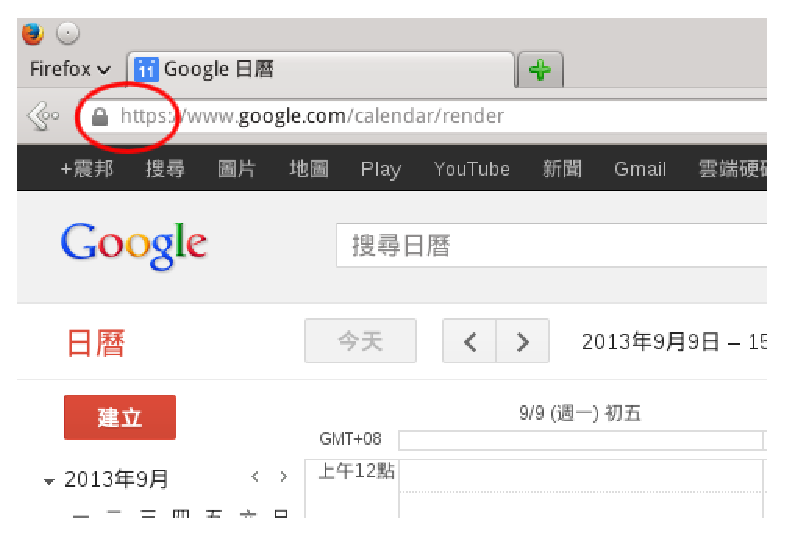
\includegraphics[scale=0.5]{https.eps}
  \end{center}
\end{frame}

\section{使用}
\subsection{權限}
\begin{frame}{共用者的權限}
  Google 日曆提供四個選項
  \begin{itemize}
    \item 進行變更並管理共用設定\only<2>{{\color{red}{(等同擁有者)}}}
    \item 變更行程
    \item 查看活動的內容
    \item 僅能查看活動的時段
  \end{itemize}
\end{frame}

\begin{frame}{對外公開的程度}
  Google 日曆提供三個選項
  \begin{itemize}
    \item
      \only<1>{公開(可搜尋)}
      \only<2>{{\color{red}{公開(可搜尋):不適合}}}
    \item 僅公開活動的時段
    \item 不公開
  \end{itemize}
\end{frame}

\subsection{調整行程}
\begin{frame}{新增行程/活動}
  \begin{center}
    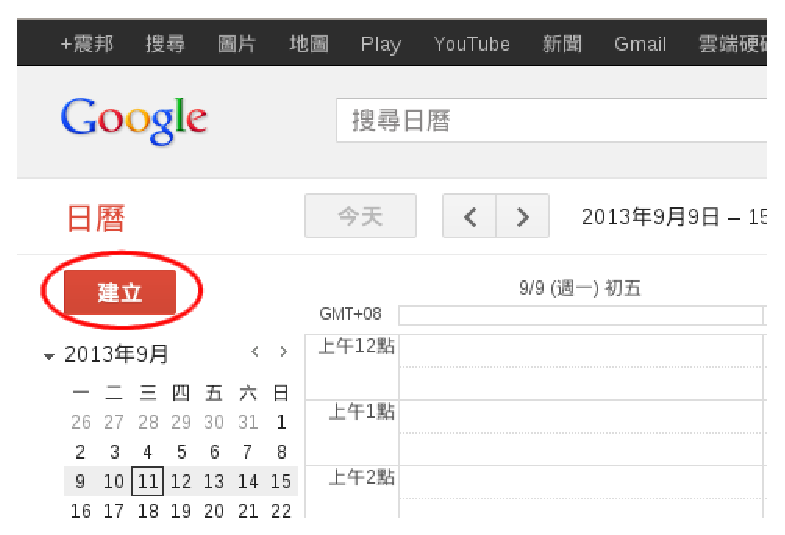
\includegraphics[scale=0.5]{create.eps}
  \end{center}
\end{frame}

\begin{frame}{編輯活動內容}
  \begin{center}
    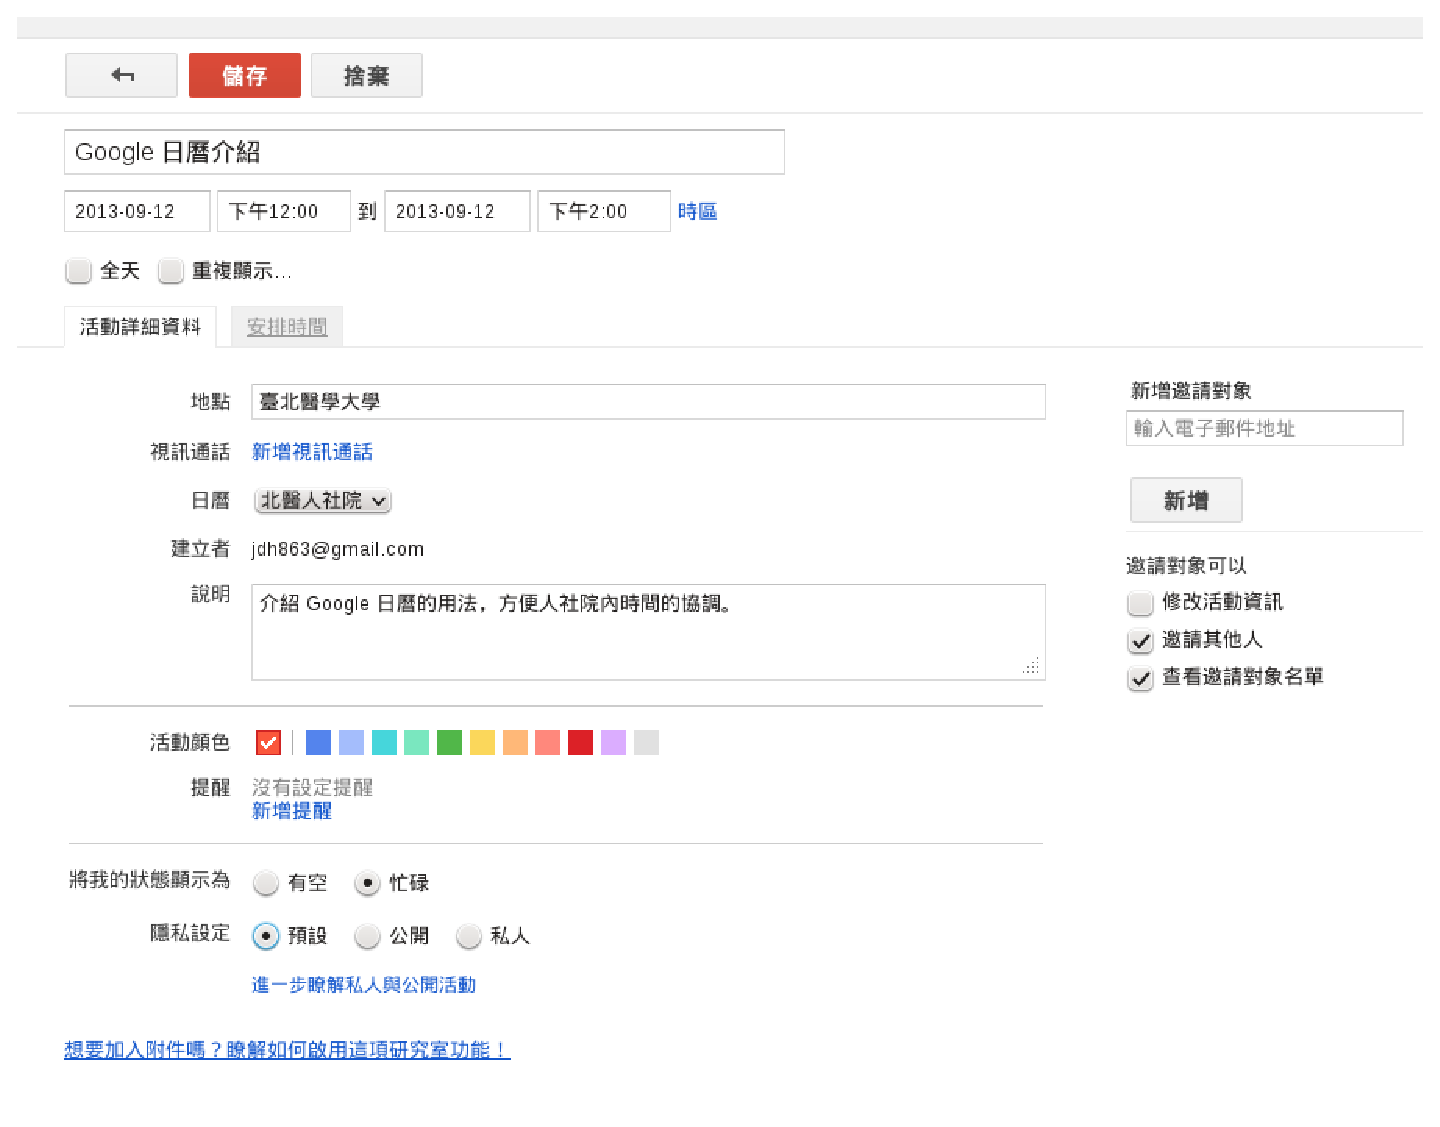
\includegraphics[scale=0.35]{edit.eps}
  \end{center}
\end{frame}

\begin{frame}{公私分明}
  \begin{center}
    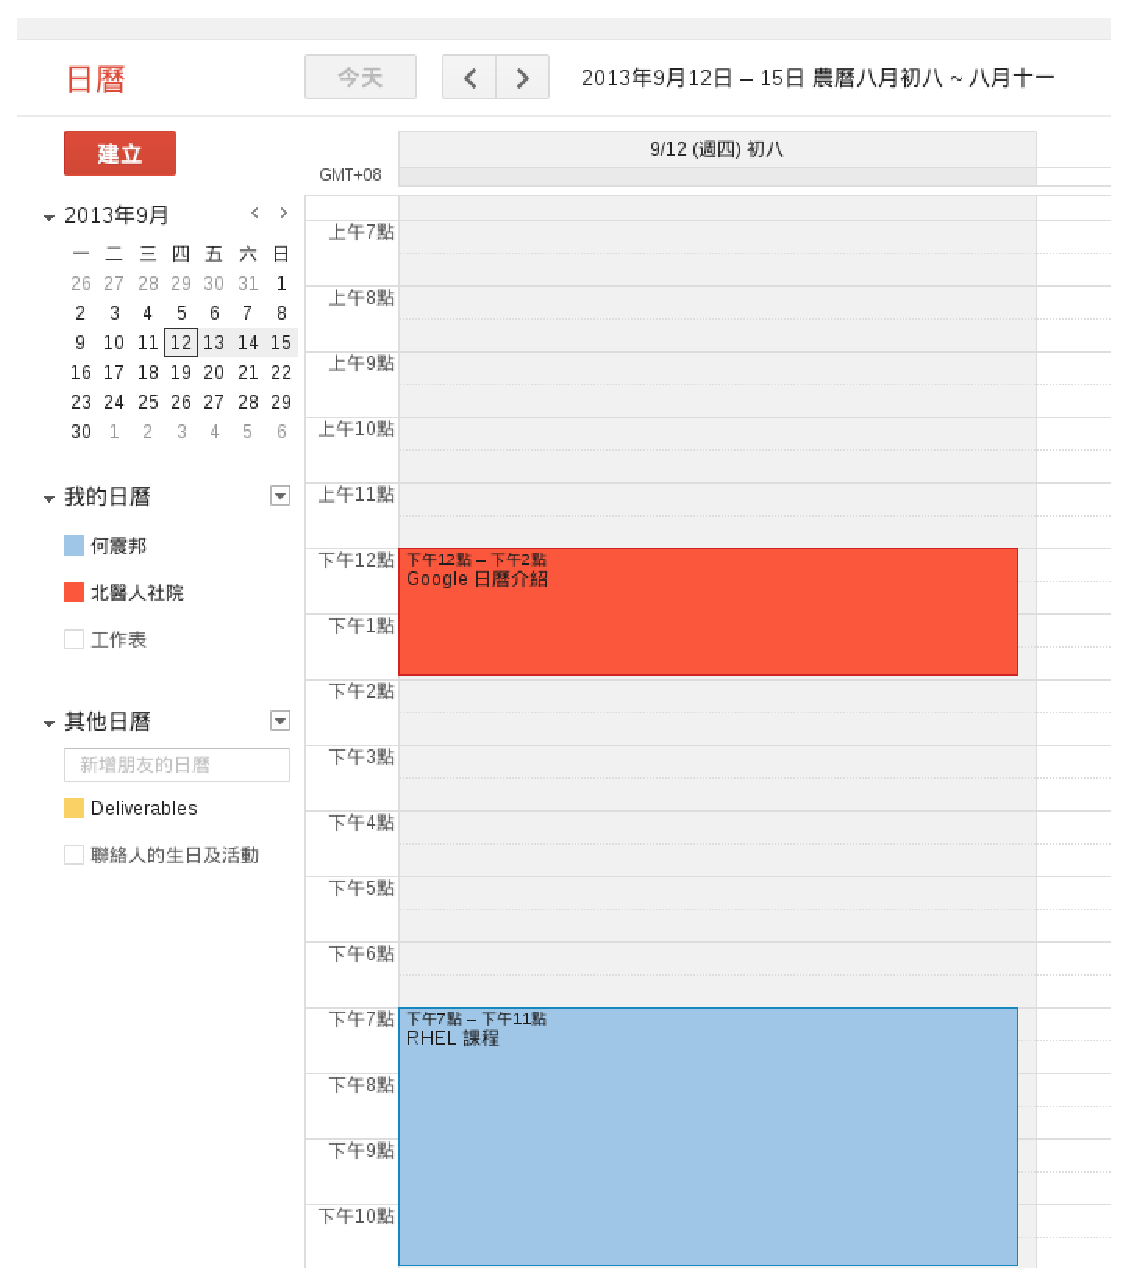
\includegraphics[scale=0.3]{clarity.eps}
  \end{center}
\end{frame}

\subsection{Demo}
\begin{frame}{Online demo}
  \begin{center}
    \href{https://www.google.com/calendar/render}{\LARGE A demo is worth a thousand words.}
  \end{center}
\end{frame}

\begin{frame}
  \begin{center}
    \huge Thanks for your attention!
  \end{center}
\end{frame}
\end{document}
